\subsection{Реляционная алгебра. Унарные и множественные операции}

В этом разделе будут описаны унарные операции в рамках реляционной алгебры. В соответствии с
определением, для определения каждой операции нужно указать способ построения заголовка, тела
отношения, а также условия применимости, если такие есть.

\subsubsection{Проекция}

\begin{definition}
	\textit{Проекцией} отношения $R$ на множество атрибутов
	$A = \{ a_1, a_2, \ldots, a_n \}$ называется отношение, полученное из исходного путем
	удаления атрибутов не из $A$. Обозначается $\pi_A(R)$.
\end{definition}

Данная операция может быть полезна для следующего:
\begin{itemize}
	\item Привести отношение к виду, в котором над ним можно будет осуществить другую операцию (например,
	      объединение);
	\item Выбрать из отношения только нужные данные (для выборки).
\end{itemize}

На рисунке \ref{proj-def} приведена иллюстрация к определению $\pi_{A_2, A_4, A_5}(A)$.

\begin{figure}[h]
	\centering
	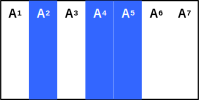
\includegraphics[width=0.8\textwidth]{../assets/kgeorgiy/relalgebra/Primitive_Projection_0.svg.png}
	\caption{Иллюстрация к определению проекции}
	\label{proj-def}
\end{figure}

Синим здесь обозначены столбцы, которые есть в результате операции. Остальные столбцы не
используются, и результат никак не зависит от их содержимого.

\paragraph{Примеры}
Приведем несколько тривиальных примеров применения проекции.

\begin{itemize}
	\item $\pi_{FirstName, LastName}$
	      \begin{figure}[H]
		      \centering
		      \includegraphics[width=0.8\textwidth]{../assets/kgeorgiy/relalgebra/Primitive_Projection_2.svg.png}
		      \caption{Проекция. Пример 1}
		      \label{proj-ex-1}
	      \end{figure}
	\item $\pi_{FirstName}$
	      \begin{figure}[H]
		      \centering
		      \includegraphics[width=0.8\textwidth]{../assets/kgeorgiy/relalgebra/Primitive_Projection_3.svg.png}
		      \caption{Проекция. Пример 2}
		      \label{proj-ex-2}
	      \end{figure}
\end{itemize}

\subsubsection{Фильтрация}

\begin{definition}
	\textit{Фильтрацией (селекцией, выборкой из)} отношения $R$ называется отношение,
	чей заголовок полностью совпадает с заголовком $R$, но тело содержит только
	кортежи, удовлетворяющее условию $c$. Обозначение: $\sigma_c(R)$.
\end{definition}

Операция часто используется для
\begin{itemize}
	\item Ограничения области действия изменяющих запросов;
	\item Получения выборки данных, соответствующих определенному условию.
\end{itemize}

На рисунке \ref{sel-def} приведена иллюстрация к определению $\sigma_c(R)$.

\begin{figure}[H]
	\centering
	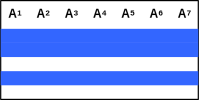
\includegraphics[width=0.8\textwidth]{../assets/kgeorgiy/relalgebra/Primitive_Section_0.svg.png}
	\caption{Иллюстрация к определению фильтрации}
	\label{sel-def}
\end{figure}

Синим здесь обозначены столбцы, которые есть в результате операции. Остальные столбцы не
используются, и результат никак не зависит от их содержимого.

\paragraph{Примеры}
Приведем несколько тривиальных примеров применения фильтрации.

\begin{itemize}
	\item $\sigma_{Id>2}$
	      \begin{figure}[H]
		      \centering
		      
\includegraphics[width=0.8\textwidth]{../assets/kgeorgiy/relalgebra/Primitive_Section_2.svg.png}
		      \caption{Фильтрация. Пример 1}
		      \label{sel-ex-1}
	      \end{figure}
	\item Можно писать более сложные условия. $\sigma_{Id>2 \wedge FirstName=\texttt{Иван}}$
	      \begin{figure}[H]
		      \centering
		      
\includegraphics[width=0.8\textwidth]{../assets/kgeorgiy/relalgebra/Primitive_Section_3.svg.png}
		      \caption{Фильтрация. Пример 2}
		      \label{sel-ex-2}
	      \end{figure}
	\item Можно использовать функции, доступные в используемой БД. \\ $\sigma_{\texttt{length}(FirstName) + 2 \geqslant \texttt{length}(LastName)}$
	      \begin{figure}[H]
		      \centering
		      \includegraphics[width=0.8\textwidth]{../assets/kgeorgiy/relalgebra/Primitive_Section_4.svg.png}
		      \caption{Фильтрация. Пример 3}
		      \label{sel-ex-3}
	      \end{figure}
\end{itemize}

\subsubsection{Переименование}\label{def-rename}

\begin{definition}
	\textit{Переименованием} называется операция, при которой меняются названия
	атрибутов отношения. Тело при этом остается неизменным.
\end{definition}

Операция часто применяется для того, чтобы отношение можно было использовать в рамках другой
операции (например, при объединении с другим отношением).

\paragraph{Примеры}
Ниже приведен тривиальный пример-пояснение для операции переименования.

\begin{itemize}
	\item $\rho_{Name=FirstName, Surname=LastName}$
	      \begin{figure}[H]
		      \centering
		      
\includegraphics[width=0.8\textwidth]{../assets/kgeorgiy/relalgebra/Primitive_Rename_2.svg.png}
		      \caption{Переименование. Пример}
		      \label{ren-ex}
	      \end{figure}
\end{itemize}

\subsubsection{Множественные операции}

Из теории множеств в реляционную алгебру естественным образом переходят операции:
\begin{itemize}
	\item $R_1 \cup R_2$ -- объединение.
	\item $R_1 \cap R_2$ -- пересечение.
	\item $R_1 \setminus R_2$ -- разность.
\end{itemize}

Эти операции по определению применимы только к отношениям с одинаковыми заголовками. В результате
получается отношение с таким же заголовком и телом, полученным в соответствии с множественной
операцией. Иначе говоря, заголовок остается тем же, а над телами отношений производится
соответствущая множественная операция (объединение, пересечение, вычитание и прочие).

\paragraph{Примеры}
\begin{itemize}
	\item Объединение отношений: $R_1 \cup R_2$
	      \begin{figure}[H]
		      \centering
		      
\includegraphics[width=0.8\textwidth]{../assets/kgeorgiy/relalgebra/Set_Union_2.svg.png}
		      \caption{Объединение отношений}
		      \label{set-union-ex}
	      \end{figure}
	\item Пересечение отношений: $R_1 \cap R_2$
	      \begin{figure}[H]
		      \centering
		      
\includegraphics[width=0.8\textwidth]{../assets/kgeorgiy/relalgebra/Set_Intersect_2.svg.png}
		      \caption{Пересечение отношений}
		      \label{set-intersect-ex}
	      \end{figure}
	\item Разность отношений: $R_1 \setminus R_2$
	      \begin{figure}[H]
		      \centering
		      
\includegraphics[width=0.8\textwidth]{../assets/kgeorgiy/relalgebra/Set_Minus_2.svg.png}
		      \caption{Разность отношений}
		      \label{set-minus-ex}
	      \end{figure}
\end{itemize}

Стоит отметить, что для объединения отношений с различающимися именами атрибутов, но при равном их
количестве, можно воспользоваться переименованием для того, чтобы привести заголовки к одному виду.
